\section{GUI}
The GUI contains following tabs:
\begin{itemize}
  \item \textbf{Enrollment} \\

    \begin{figure}[H]
      \centering
      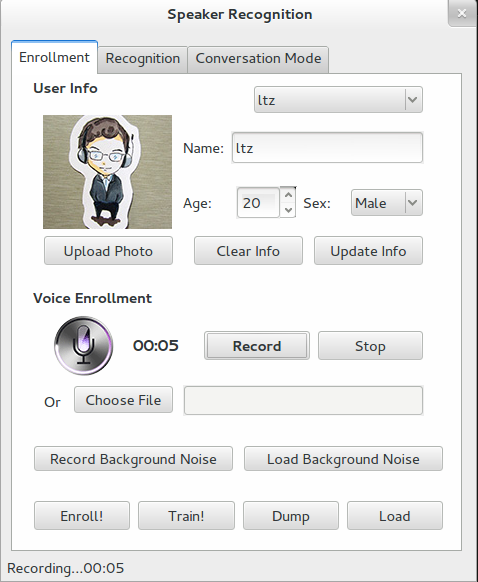
\includegraphics[width=0.8\textwidth]{img/enrollment.png}
    \end{figure}

    A new user may start his or her first step by clicking the
    tab Enrollment. New users could provide personal information
    such as name, sex, and age. then upload personal avatar to
    build up their own data. Experienced users can choose from
    the userlist and update their infomation.

    Next the user needs to provide a piece of utterance for
    the enrollment and training process.

    There are two ways to enroll a user:
    \begin{itemize}
      \item \textbf{Enroll by Recording}
        Click Record and start talking while click Stop to stop
        and save.There is no limit of the content of the utterance,
        whileit is highly recommended that the user speaks long enough
        to provide sufficient message for the enrollment.

      \item \textbf{Enroll from Wav Files}
        User can upload a pre-recorded voice of a speaker.(*.wav recommended)
        The systemaccepts the voice given and the enrollment of a speaker is done.
    \end{itemize}

    The user can train, dump or load his/her voice features after enrollment.

  \item \textbf{Recognition of a user} \\
    \begin{figure}[H]
      \centering
      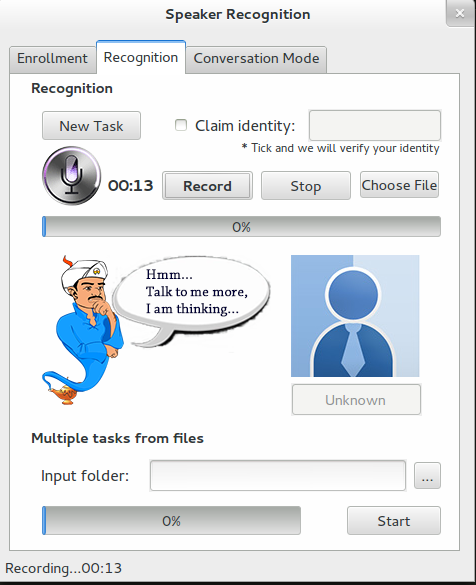
\includegraphics[width=0.8\textwidth]{img/recognition.png}
    \end{figure}

    A enrolled user present or record a piece of utterance,
    the system tells who the person is and show user's avatar.
    Recognition of multiple pre-recorded files can be done as well.

  \item \textbf{Conversation Recognition Mode} \\
    \begin{figure}[H]
      \centering
      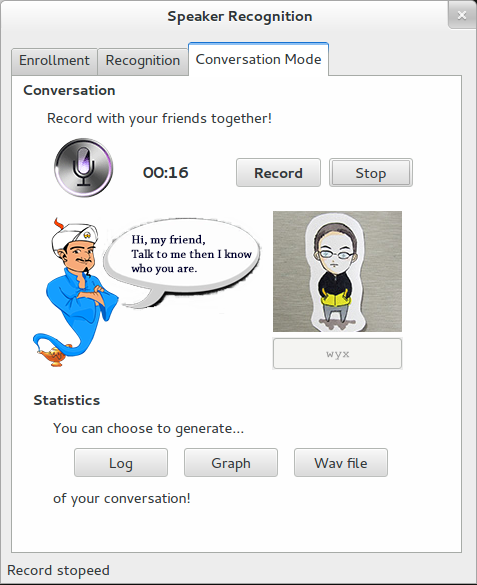
\includegraphics[width=0.8\textwidth]{img/conversation.png}
      \caption{\label{fig:}}
    \end{figure}

    In Conversation Recognition mode, multiple users can have conversations
    together near the microphone. Same recording procedure as above.
    The system will continuously collect voice data, and determine
    who is speaking right now. Current speaker's anvatar will show up
    in screen; otherwise the name will be shown. The conversation
    audio can be downloaded and saved.
    There are some ways to visualize the speaker-distribution in the
    conversation.
    \begin{itemize}
      \item \textbf{Conversation log}
        A detailed log, including start time, stop time,
        current speaker of each period is generated.
      \item \textbf{Conversation flow graph}
        \begin{figure}[H]
          \centering
          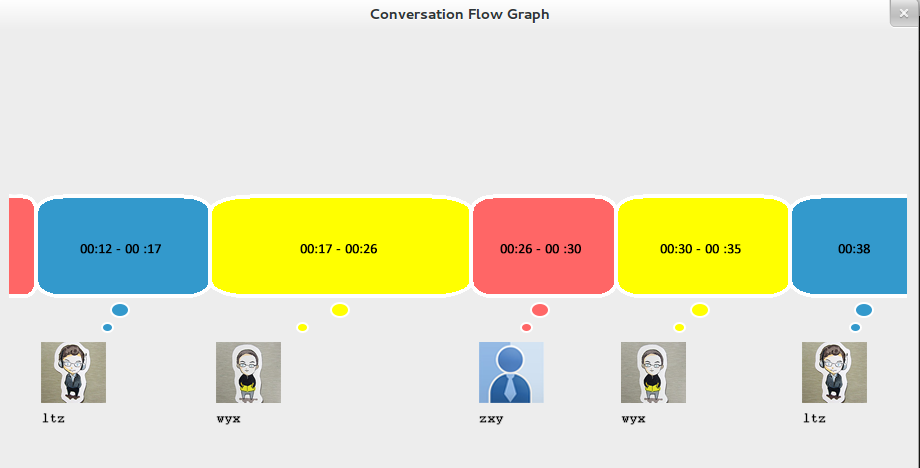
\includegraphics[width=0.8\textwidth]{img/conversationgraph.png}
        \end{figure}

        A timeline of the conversation will be shown by a number of
        talking-clouds joining together, with start time, stop time
        and users' avatars labeled. Different users are presented
        with different colors.The timeline will flow to the left dynamically
        just as time elapses. The visualization of the conversation is done
        in this way. This functionality is still under development.
    \end{itemize}

\end{itemize}
